\begin{figure}[htbp]
    \centering
    \begin{subfigure}[tb]{0.45\textwidth}
        \centering
        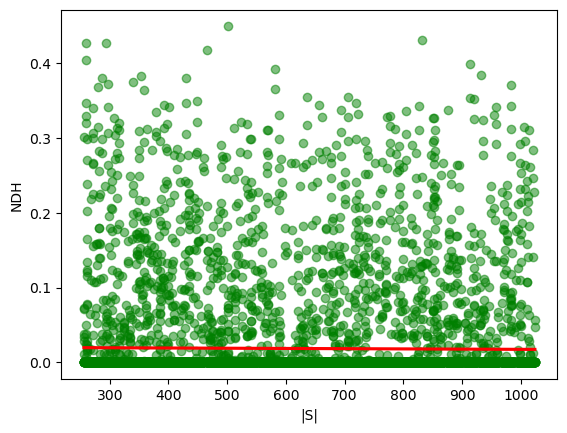
\includegraphics[width=\textwidth]{metrics/size_ndh.png}
        \caption{No correlation between the number of states in the environment and \textbf{NDH metric}: $y = -0.0x  + 0.009, R^2 = 0.005, p < 10^{-8}$.}
        \label{fig: dropvsdist}
    \end{subfigure}
    \hfill
    \begin{subfigure}[tb]{0.45\textwidth}
        \centering
        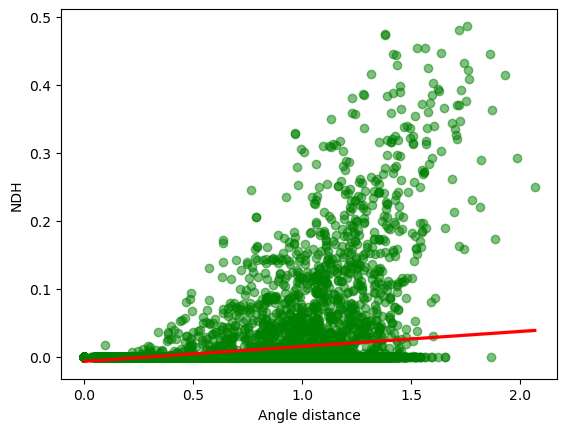
\includegraphics[width=\textwidth]{metrics/distance_ndh.png}
        \caption{Weak anti-correlation between the cosine similarity and \textbf{NDH metric}: $y = -0.03x  + -0.004, R^2 = 0.038, p < 10^{-8}$.}
        \label{fig: dropvsdims}
    \end{subfigure}
    \hfill
    \begin{subfigure}[tb]{0.45\textwidth}
        \centering
        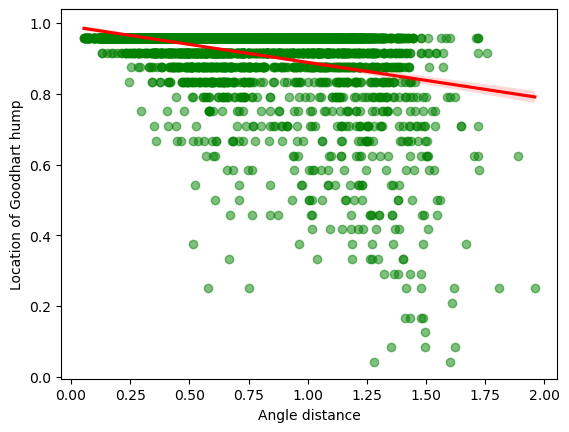
\includegraphics[width=\textwidth]{metrics/goodhart_hump_location.png}
        \caption{Weak anti-correlation between the distance to the proxy reward, and the \textbf{location of the Goodhart's hump}: $y = -0.19x  + 0.98, R^2 = 0.09, p < 10^{-8}$.}
        \label{fig:goodharting-distance}
    \end{subfigure}
    \hfill
    \begin{subfigure}[tb]{0.45\textwidth}
        \centering
        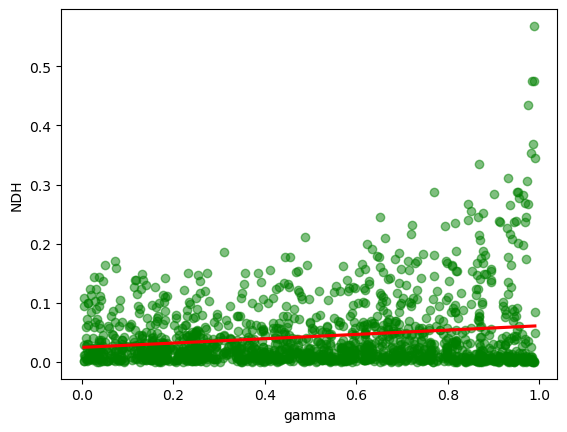
\includegraphics[width=\textwidth]{metrics/gamma_ndh.png}
        \caption{Weak positive correlation between $\gamma$ and the \textbf{NDH metric}: $y = -0.19x  + 0.98, R^2 = 0.09, p < 10^{-8}$.}
        \label{fig:goodharting-distance}
    \end{subfigure}
    \hfill
    \begin{subfigure}[tb]{0.45\textwidth}
        \centering
        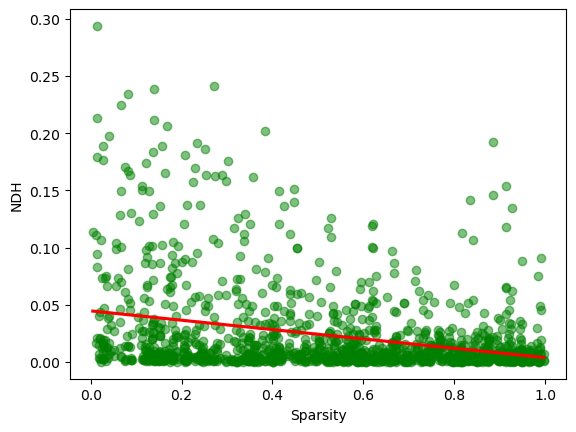
\includegraphics[width=\textwidth]{metrics/sparsity_ndh.png}
        \caption{Weak anti-correlation between the sparsity of the reward, and the \textbf{NDH metric}: $y = -0.19x  + 0.98, R^2 = 0.09, p < 10^{-8}$.}
        \label{fig:goodharting-distance}
    \end{subfigure}
    \hfill
    \begin{subfigure}[tb]{0.45\textwidth}
        \centering
        \includegraphics[width=\textwidth]{metrics/envtype_ndh.png}
        \caption{Goodhart's effect size in different types of environments.}
        \label{fig:goodharting-distance}
    \end{subfigure}
    \caption{Correlation between something something.}
    \label{fig:goodhart-trends}
\end{figure}
